\chapter{Üzembe helyezés és kísérleti eredmények}
\label{chap:uzembehelyezes}

Ez a fejezet bemutatja a rendszer üzembe helyezésének gyakorlati lépéseit, a szoftver fejlesztése és futtatása során felmerült technikai problémákat és azok megoldásait, valamint a betanított modellekkel végzett kísérletek és mérések számszerűsített eredményeit.

\section{Üzembe helyezési lépések}
\label{sec:uzembehelyezes}

A hangszerfelismerő rendszer két fő részből áll: a háttérben futó gépi tanulási és jelfeldolgozó modulokból, valamint a valós idejű parancssori felhasználói alkalmazásból (CLI Dashboard). A szoftver üzembe helyezéséhez az alábbi lépések szükségesek:

\begin{enumerate}
    \item \textbf{Python környezet előkészítése:} A futtatáshoz legalább Python 3.10 verzió szükséges. Ajánlott egy izolált virtuális környezet (virtual environment) létrehozása a függőségek kezelésére:
\begin{verbatim}
python3 -m venv venv
source venv/bin/activate
\end{verbatim}

    \item \textbf{Rendszerszintű függőségek telepítése:} A valós idejű hangrögzítésért felelős \texttt{sounddevice} könyvtár a PortAudio C-könyvtárra épül. macOS rendszereken ezt a Homebrew segítségével kell telepíteni:
\begin{verbatim}
brew install portaudio
\end{verbatim}
    Windows és Linux platformokon a csomagkezelők többsége automatikusan fordítja vagy tartalmazza a szükséges binárisokat.

    \item \textbf{Python könyvtárak telepítése:} A szükséges csomagok listáját a \texttt{requirements.txt} tartalmazza. Telepítésük a következő paranccsal végezhető el:
\begin{verbatim}
pip install -r requirements.txt
\end{verbatim}
    A legfontosabb telepített csomagok: \texttt{tensorflow} (neurális hálózat futtatása), \texttt{librosa} (jellemzőkinyerés), \texttt{sounddevice} (mikrofonkezelés), valamint a vizualizációért felelős \texttt{matplotlib} és \texttt{numpy}.

    \item \textbf{Modellfájlok elhelyezése:} A betanított neurális hálózati modelleket a \texttt{best\_log\_mel\_}\allowbreak\texttt{2dcnn\_model.keras} és a \texttt{best\_stft\_}\allowbreak\texttt{2dcnn\_model.keras} fájlok formájában a projekt \texttt{models/} alkönyvtárába kell elhelyezni.

    \textbf{}
    \item \textbf{Alkalmazás indítása:} A valós idejű parancssori felület az alábbi parancs futtatásával indítható el:
\begin{verbatim}
python scripts/07_realtime_recognition.py
\end{verbatim}
\end{enumerate}

\section{Felmerült problémák és megoldások}
\label{sec:problemak}

\section{Kísérleti eredmények és mérések}
\label{sec:kiserletek}

A legjobb eredményt nyújtó Log-Mel alapú modell hangszerenkénti osztályozási mátrixát (konfúziós mátrix) vizsgáltam meg részletesebben. A~\ref{fig:confusion_matrix}.~ábra hőtérkép (heatmap) formájában mutatja a hangszerosztályok közötti tévesztési arányokat és a pontos mintaszámokat az osztályozás során.

\begin{figure}[H]
  \centering
  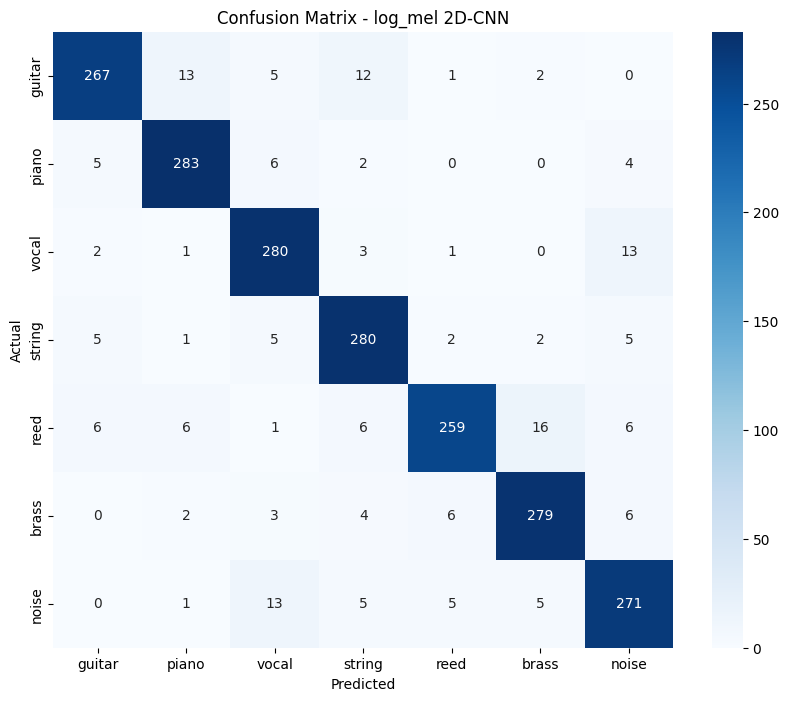
\includegraphics[width=0.8\textwidth]{fig_confusion_matrix.png}
  \caption{A Log-Mel spektrogram alapú 2D CNN modell konfúziós mátrixának hőtérképe}
  \label{fig:confusion_matrix}
\end{figure}

A konfúziós mátrix hőtérképéből leolvasható, hogy a legkönnyebben és legbiztosabban felismerhető kategória a \texttt{Zongora} (94,3\%, azaz 283 helyes predikció a 300 tesztmintából), valamint az \texttt{Ének} és a \texttt{Vonósok} (mindkettő 93,3\%, azaz 280/300 helyes osztályozás). A zongora tiszta leütési tranziensei és a vonósok egyenletes, hosszan tartó harmonikus felhangszerkezete jól elkülöníthető vizuális mintázatot adnak a Log-Mel spektrogramon, miközben az énekhang egyedi formánsai (a vokális traktus rezonanciája) szintén markáns ujjlenyomatként jelennek meg.

A legnagyobb arányú tévesztések a következők szerint alakultak:
\begin{itemize}
    \item \textbf{Fúvós hangszerek:} A \texttt{Nádas} fúvósok mintáinak 5,3\%-át (16 mintát) a modell \texttt{Rézfúvósnak} osztályozta. Ez a tévesztés akusztikailag rendkívül indokolt, mivel például az egynádas szaxofon (nádas fúvós) és a trombita (rézfúvós) felhangszerkezete és megszólalási tranziensei bizonyos hangmagasságoknál nagyon hasonlóak.
    \item \textbf{Zongora és Gitár:} A \texttt{Gitár} minták 4,3\%-át (13 mintát) a modell \texttt{Zongorának} osztályozta. Ez a pengetett és leütött húrok fizikai rezgésének kezdeti lecsengési hasonlóságából fakad, különösen az akusztikus gitár esetében.
    \item \textbf{Ének és Háttérzaj:} A \texttt{Háttérzaj} minták 4,3\%-át (13 mintát) \texttt{Éneknek}, míg az \texttt{Ének} minták 4,3\%-át (13 mintát) \texttt{Háttérzajnak} jelölte a hálózat. Ez a mikrofonos zörejek, zihálások és az emberi beszéd/ének frekvenciatartományának átfedései miatt fordul elő, valamint a halkabb énekszakaszok és a környezeti zajok hasonlóságából adódik.
\end{itemize}
Mintent összevetve a Log-Mel alapú 2D CNN modell kiválóan teljesít: a legnehezebbnek bizonyuló \texttt{Nádas} osztályban is eléri a 86,3\%-os pontosságot, míg a többi zenei és környezeti kategóriában 89\% feletti egyedi pontosságot biztosít.
